\documentclass{article}

% if you need to pass options to natbib, use, e.g.:
%     \PassOptionsToPackage{numbers, compress}{natbib}
% before loading neurips_2025

% The authors should use one of these tracks.
% Before accepting by the NeurIPS conference, select one of the options below.
% 0. "default" for submission
 \usepackage[main, final]{nthu_nlp_final_2025}
% the "default" option is equal to the "main" option, which is used for the Main Track with double-blind reviewing.
% 1. "main" option is used for the Main Track
%  \usepackage[main]{neurips_2025}
% 2. "position" option is used for the Position Paper Track
%  \usepackage[position]{neurips_2025}
% 3. "dandb" option is used for the Datasets & Benchmarks Track
 % \usepackage[dandb]{neurips_2025}
% 4. "creativeai" option is used for the Creative AI Track
%  \usepackage[creativeai]{neurips_2025}
% 5. "sglblindworkshop" option is used for the Workshop with single-blind reviewing
 % \usepackage[sglblindworkshop]{neurips_2025}
% 6. "dblblindworkshop" option is used for the Workshop with double-blind reviewing
%  \usepackage[dblblindworkshop]{neurips_2025}

% After being accepted, the authors should add "final" behind the track to compile a camera-ready version.
% 1. Main Track
 % \usepackage[main, final]{neurips_2025}
% 2. Position Paper Track
%  \usepackage[position, final]{neurips_2025}
% 3. Datasets & Benchmarks Track
 % \usepackage[dandb, final]{neurips_2025}
% 4. Creative AI Track
%  \usepackage[creativeai, final]{neurips_2025}
% 5. Workshop with single-blind reviewing
%  \usepackage[sglblindworkshop, final]{neurips_2025}
% 6. Workshop with double-blind reviewing
%  \usepackage[dblblindworkshop, final]{neurips_2025}
% Note. For the workshop paper template, both \title{} and \workshoptitle{} are required, with the former indicating the paper title shown in the title and the latter indicating the workshop title displayed in the footnote.
% For workshops (5., 6.), the authors should add the name of the workshop, "\workshoptitle" command is used to set the workshop title.
% \workshoptitle{WORKSHOP TITLE}

% "preprint" option is used for arXiv or other preprint submissions
 % \usepackage[preprint]{neurips_2025}

% to avoid loading the natbib package, add option nonatbib:
%    \usepackage[nonatbib]{neurips_2025}

\usepackage[utf8]{inputenc} % allow utf-8 input
\usepackage[T1]{fontenc}    % use 8-bit T1 fonts
\usepackage{hyperref}       % hyperlinks
\usepackage{url}            % simple URL typesetting
\usepackage{booktabs}       % professional-quality tables
\usepackage{amsfonts}       % blackboard math symbols
\usepackage{amsmath}        % for \text command in equations
\usepackage{nicefrac}       % compact symbols for 1/2, etc.
\usepackage{microtype}      % microtypography
\usepackage{xcolor}         % colors
\usepackage{graphicx}       % images
\usepackage{tikz}           % diagrams
\usepackage{fontawesome5}   % icons (GitHub)
\usetikzlibrary{shapes.geometric, arrows, positioning, fit, backgrounds}
\graphicspath{ {images/} }

% Note. For the workshop paper template, both \title{} and \workshoptitle{} are required, with the former indicating the paper title shown in the title and the latter indicating the workshop title displayed in the footnote. 
\title{Soft Spearman Loss for \\ Subjective Q\&A Quality Estimation \\ 
\vspace{2mm} \large A Solution for the Google QUEST Challenge}


% The \author macro works with any number of authors. There are two commands
% used to separate the names and addresses of multiple authors: \And and \AND.
%
% Using \And between authors leaves it to LaTeX to determine where to break the
% lines. Using \AND forces a line break at that point. So, if LaTeX puts 3 of 4
% authors names on the first line, and the last on the second line, try using
% \AND instead of \And before the third author name.


\author{%
  Shu-wen Yang \quad Yi-Cheng Lin \quad Leonardo Haw-Yang Foo \\
  National Taiwan University, Taiwan \\
  \textit{Team NTU SPML}
}


\begin{document}


\maketitle


\begin{abstract}
  We present a solution for the Google QUEST Q\&A Labeling challenge that systematically improves upon a competitive baseline (23rd place). By adopting DeBERTa-v3-Large, we leverage its disentangled attention mechanism, which separates content and positional representations for improved long-range dependency modeling. Extending the maximum sequence length to 1024 tokens mitigates the context truncation observed in the baseline. To address the label noise inherent in subjective human ratings, we replace the standard Binary Cross Entropy (BCE) loss with a ranking-aware objective augmented by a differentiable Soft Spearman loss. Finally, we employ a two-phase training strategy to stabilize learning of question-specific representations. Our final model achieves a Cross-Validation Spearman correlation of 0.4228, outperforming the baseline (0.4195). These results underscore the importance of ranking-oriented objectives for subjective quality estimation.
\end{abstract}

\noindent Our code is publicly available at \url{https://github.com/leonardofhy/google_quest_qa_labeling}.


\section{Task Description}

The Google QUEST Q\&A Labeling competition [11] tasks participants with predicting human-annotated quality scores for question-answer pairs sourced from StackExchange. These scores capture diverse subjective dimensions of Q\&A quality.

\subsection{Problem Definition}
The task is formulated as multi-output regression. Each sample comprises a question title, question body, and answer. The output is a vector of 30 scalar values in $[0, 1]$, each corresponding to a distinct quality dimension. These dimensions span two categories:
\begin{enumerate}
    \item \textbf{Question Ratings}: 21 dimensions evaluating the question's intent, type (e.g., instructional, conversational), and quality (e.g., well-written, helpful).
    \item \textbf{Answer Ratings}: 9 dimensions evaluating the answer's quality (e.g., helpfulness, plausibility, level of detail).
\end{enumerate}

\subsection{Evaluation Metric}
Performance is measured by the \textbf{Spearman rank correlation coefficient}. For each of the 30 target dimensions, the Spearman correlation between predictions and ground truth is computed; the final score is the mean across all dimensions. This metric prioritizes relative ranking over absolute values, posing a challenge for standard regression losses such as Mean Squared Error (MSE) and Binary Cross Entropy (BCE).

\subsection{Key Challenges}
\begin{itemize}
    \item \textbf{Subjectivity}: Labels are derived from human annotators and reflect subjective judgments, introducing inherent label noise.
    \item \textbf{Data Scarcity}: With approximately 6,000 training and fewer than 500 test samples, the dataset poses a significant overfitting risk.
    \item \textbf{Ranking Sensitivity}: The Spearman metric requires correct relative ordering of predictions, making it sensitive to distribution shifts and necessitating ranking-aware optimization.
\end{itemize}




\section{Related Work}

\subsection{Baseline Overview}
We adopt the 23rd-place solution from the Kaggle competition as our baseline. This solution employs \texttt{bert-base-uncased} [2] with a maximum sequence length of 512 tokens. A notable design choice is its pooling strategy: concatenating the \texttt{[CLS]} and \texttt{[SEP]} token embeddings from the last four hidden layers.

Training employs a \textbf{Ranking + Binary Cross Entropy (BCE)} loss. To mitigate overfitting, the baseline adopts a two-phase training strategy: the model first trains on question title and body to learn robust question representations, then fine-tunes on complete Q\&A pairs. Post-processing includes stacking via LightGBM [10].

\subsection{Baseline Analysis}
Table \ref{tab:comparison} summarizes the differences between the baseline and our approach.

\begin{table}[h]
  \caption{Comparison between the baseline and our proposed approach.}
  \label{tab:comparison}
  \centering
  \begin{tabular}{lcc}
    \toprule
    \textbf{Aspect} & \textbf{Baseline (23rd)} & \textbf{Ours} \\
    \midrule
    Backbone & BERT-Base (110M) & DeBERTa-v3-Large (435M) \\
    Sequence Length & 512 & 1024 \\
    Pooling & [CLS] + [SEP] (Last 4 layers) & WLP + Attention \\
    Loss Function & Ranking + BCE & Ranking + Soft Spearman \\
    Ensembling & 30 Snapshots & Single Model \\
    \bottomrule
  \end{tabular}
\end{table}

The baseline's primary limitation is its reliance on BERT's 512-token context window, leading to truncation of longer Q\&A pairs. Furthermore, while BCE serves as a reasonable regression surrogate, it does not directly optimize the Spearman correlation used for evaluation.

\section{Methods}
We introduce four key improvements over the baseline: (1) a more expressive backbone architecture, (2) an enhanced pooling strategy, (3) extended context length, and (4) a ranking-aware optimization objective.

\subsection{Model Architecture}
We replace the BERT backbone with DeBERTa-v3-Large [1]. DeBERTa employs a disentangled attention mechanism that decouples content and positional representations, enabling more effective modeling of long-range dependencies between questions and answers.
Figure~\ref{fig:architecture} illustrates our model architecture.

\begin{figure}[h]
    \centering
    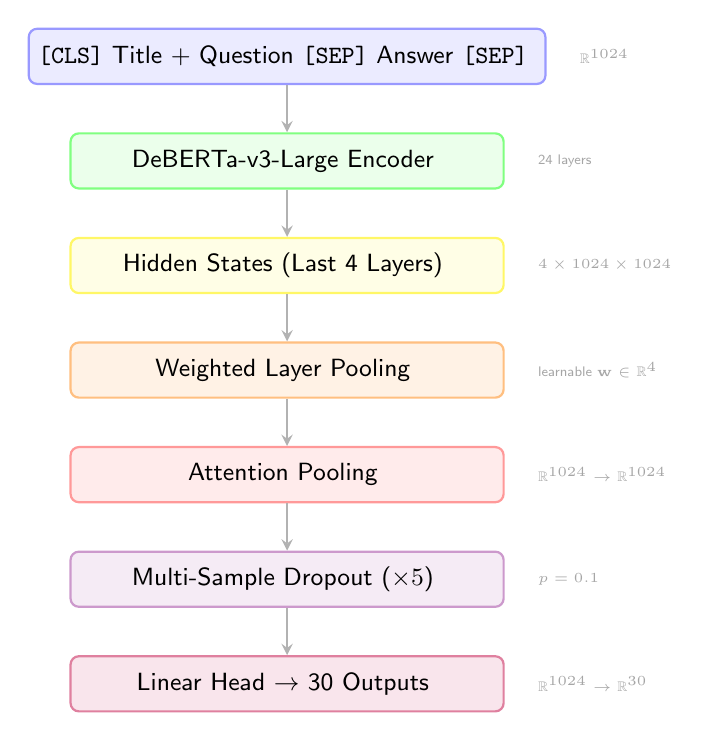
\begin{tikzpicture}[
        node distance=0.6cm,
        % Main component boxes
        mainbox/.style={
            rectangle, draw=gray!70, rounded corners=3pt, 
            minimum width=5.5cm, minimum height=0.7cm, 
            align=center, font=\small\sffamily,
            line width=0.8pt
        },
        % Annotation style
        annot/.style={font=\tiny\sffamily\color{gray!70}, align=left},
        % Arrow style
        arrow/.style={->, >=stealth, thick, draw=gray!60}
    ]
        % Input Layer
        \node[mainbox, fill=blue!8, draw=blue!40] (input) {
            \texttt{[CLS]} Title + Question \texttt{[SEP]} Answer \texttt{[SEP]}
        };
        \node[annot, right=0.3cm of input] {$\mathbb{R}^{1024}$};
        
        % Encoder
        \node[mainbox, fill=green!8, draw=green!50, below=of input] (encoder) {
            DeBERTa-v3-Large Encoder
        };
        \node[annot, right=0.3cm of encoder] {24 layers};
        
        % Hidden states with visual representation
        \node[mainbox, fill=yellow!10, draw=yellow!60, below=of encoder] (hidden) {
            Hidden States (Last 4 Layers)
        };
        \node[annot, right=0.3cm of hidden] {$4 \times 1024 \times 1024$};
        
        % Weighted Layer Pooling
        \node[mainbox, fill=orange!10, draw=orange!50, below=of hidden] (wlp) {
            Weighted Layer Pooling
        };
        \node[annot, right=0.3cm of wlp] {learnable $\mathbf{w} \in \mathbb{R}^4$};
        
        % Attention Pooling
        \node[mainbox, fill=red!8, draw=red!40, below=of wlp] (attn) {
            Attention Pooling
        };
        \node[annot, right=0.3cm of attn] {$\mathbb{R}^{1024} \rightarrow \mathbb{R}^{1024}$};
        
        % Multi-Sample Dropout
        \node[mainbox, fill=violet!8, draw=violet!40, below=of attn] (dropout) {
            Multi-Sample Dropout ($\times 5$)
        };
        \node[annot, right=0.3cm of dropout] {$p=0.1$};
        
        % Output Head
        \node[mainbox, fill=purple!10, draw=purple!50, below=of dropout] (output) {
            Linear Head $\rightarrow$ 30 Outputs
        };
        \node[annot, right=0.3cm of output] {$\mathbb{R}^{1024} \rightarrow \mathbb{R}^{30}$};
        
        % Arrows with clean styling
        \draw[arrow] (input) -- (encoder);
        \draw[arrow] (encoder) -- (hidden);
        \draw[arrow] (hidden) -- (wlp);
        \draw[arrow] (wlp) -- (attn);
        \draw[arrow] (attn) -- (dropout);
        \draw[arrow] (dropout) -- (output);
        
    \end{tikzpicture}
    \caption{Model architecture overview. Input tokens are encoded by DeBERTa-v3-Large, and hidden states from the last four layers are aggregated via Weighted Layer Pooling. Attention Pooling subsequently produces a fixed-dimensional representation. Multi-Sample Dropout [9] with 5 masks (averaged) is applied before the linear prediction head.}
    \label{fig:architecture}
\end{figure}



\subsection{Pooling Strategy}
In contrast to the baseline's \texttt{[CLS]}+\texttt{[SEP]} concatenation, we employ \textbf{Weighted Layer Pooling} followed by \textbf{Attention Pooling}. Hidden states from the last four encoder layers are first aggregated via a learnable weighted average. The resulting token embeddings are subsequently processed by an Attention Pooling layer, which assigns learned attention weights to tokens based on their informativeness, producing a fixed-dimensional representation for downstream prediction.

\subsection{Context Length Extension}
The baseline's 512-token limit constitutes a significant bottleneck, as longer Q\&A pairs are truncated and critical context is lost. We extend the maximum sequence length to \textbf{1,024 tokens}, enabling the model to attend to complete question bodies and answers simultaneously. This extension is particularly beneficial for evaluating dimensions such as ``level\_of\_detail'' and ``relevance,'' which inherently require access to the complete textual context.

\subsection{Optimization Objectives}
The evaluation metric, Spearman rank correlation, depends on the relative ordering of predictions rather than their absolute values. The baseline employs a combined Ranking and BCE loss: while the ranking component aligns with this metric, BCE penalizes absolute prediction error, which is suboptimal given the inherent noise in subjective human annotations. We therefore discard the BCE term ($\lambda_{\text{bce}}=0$) and instead optimize a weighted combination of Ranking Loss and \textbf{Soft Spearman Loss}---a differentiable approximation of Spearman correlation inspired by Blondel et al.\ [4]---enabling direct optimization of the evaluation metric.

The Soft Spearman Loss approximates discrete ranking via a sigmoid-based differentiable soft rank function:
\begin{equation}
    r_i^{\text{soft}} = \sum_{j} \sigma\left(\frac{x_i - x_j}{\tau}\right)
\end{equation}
where $\tau$ is a temperature parameter controlling approximation sharpness, $x_i$ and $x_j$ denote prediction scores, and $\sigma(\cdot)$ is the sigmoid function. The loss is defined as:
\begin{equation}
    \mathcal{L}_{\text{soft-spearman}} = 1 - \rho(r^{\text{soft}}_{\text{pred}}, r^{\text{soft}}_{\text{target}})
\end{equation}
where $\rho$ denotes Pearson correlation computed over soft ranks.
The overall training objective is formulated as a weighted sum of these ranking-aware loss components:
\begin{equation}
    \mathcal{L} = \lambda_{\text{rank}} \mathcal{L}_{\text{ranking}} + \lambda_{\text{spearman}} \mathcal{L}_{\text{soft-spearman}}
\end{equation}


\subsection{Training Strategy}
We retain the baseline's \textbf{two-phase training} strategy, as illustrated in Figure~\ref{fig:two_phase}. In Phase~1, the model is trained on question-only data (title and body) to establish robust question representations. In Phase~2, training continues on complete Q\&A pairs, incorporating all 30 target dimensions. During ablation experiments (Exp~0--3), we use 3 epochs per phase; the final configuration extends this to 5 epochs per phase to improve model stability and convergence.

\begin{figure}[h]
    \centering
    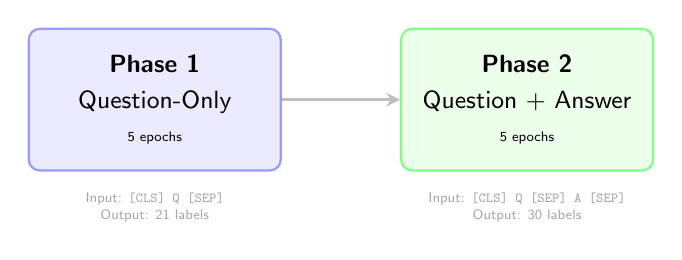
\begin{tikzpicture}[
        phase/.style={
            rectangle, draw=gray!70, rounded corners=4pt,
            minimum width=3.2cm, minimum height=1.8cm,
            align=center, font=\small\sffamily,
            line width=0.8pt
        },
        label/.style={font=\footnotesize\sffamily\bfseries},
        detail/.style={font=\tiny\sffamily, text=gray!70, align=center},
        arrow/.style={->, >=stealth, very thick, draw=gray!50}
    ]
        % Phase 1
        \node[phase, fill=blue!8, draw=blue!40] (p1) {
            \textbf{Phase 1}\\[2pt]
            Question-Only\\[1pt]
            {\tiny 5 epochs}
        };
        \node[detail, below=0.15cm of p1] (p1detail) {
            Input: \texttt{[CLS] Q [SEP]}\\
            Output: 21 labels
        };
        
        % Phase 2
        \node[phase, fill=green!8, draw=green!50, right=1.5cm of p1] (p2) {
            \textbf{Phase 2}\\[2pt]
            Question + Answer\\[1pt]
            {\tiny 5 epochs}
        };
        \node[detail, below=0.15cm of p2] (p2detail) {
            Input: \texttt{[CLS] Q [SEP] A [SEP]}\\
            Output: 30 labels
        };
        
        % Arrow
        \draw[arrow] (p1.east) -- (p2.west);
        
    \end{tikzpicture}
    \caption{Two-phase training strategy. Phase~1 trains on question context only (predicting 21 question-related dimensions) to establish robust question representations. Phase~2 fine-tunes on complete Q\&A pairs (predicting all 30 dimensions). Epoch counts: 3+3 for Exp~0--3; 5+5 for Final.}
    \label{fig:two_phase}
\end{figure}



\section{Experiments}

\subsection{Experimental Setup}
We employ 5-fold cross-validation on the training set for model evaluation. Optimization is performed using AdamW [5] with layer-wise learning rate decay ($\gamma = 0.9$). Hyperparameter settings are summarized in Table~\ref{tab:hyperparams}.

\begin{table}[h]
  \caption{Hyperparameter settings for all experiments. $^\dagger$Exp~0--3 use 3 epochs; Final uses 5 epochs.}
  \label{tab:hyperparams}
  \centering
  \begin{tabular}{lc}
    \toprule
    \textbf{Hyperparameter} & \textbf{Value} \\
    \midrule
    Max Sequence Length & 1024 \\
    Batch Size & 8 \\
    Gradient Accumulation Steps & 2 \\
    Encoder Learning Rate & $1 \times 10^{-5}$ \\
    Head Learning Rate & $1 \times 10^{-4}$ \\
    Weight Decay & $1 \times 10^{-2}$ \\
    Layer Decay ($\gamma$) & 0.9 \\
    $\lambda_{\text{rank}}$ & 1.0 \\
    $\lambda_{\text{spearman}}$ & 0.5 \\
    Spearman Temperature ($\tau$) & 0.1 \\
    Phase 1 Epochs & 3 / 5$^\dagger$ \\
    Phase 2 Epochs & 3 / 5$^\dagger$ \\
    \bottomrule
  \end{tabular}
\end{table}

\subsection{Results}
Table~\ref{tab:results} presents experimental results, reporting Cross-Validation (CV) and Kaggle Leaderboard (LB) Spearman correlation scores. The BERT-base baseline serves as our reference point. An initial configuration (Exp~0)---migrating to DeBERTa-Base with modified preprocessing and pooling while retaining the 512-token context limit---resulted in substantial performance degradation. This degradation likely stems from multiple simultaneous changes during the migration process, which we analyze below.

Extending the sequence length to 1024 tokens (Exp~1) yielded immediate performance recovery (+0.0155), confirming context length as a primary bottleneck. Incorporating the Ranking Loss and Soft Spearman Loss (Exp~2) produced the largest single improvement (+0.0229), underscoring the importance of metric-aligned optimization. Scaling to DeBERTa-v3-Large (Exp~3) and extending the training schedule to 5+5 epochs (Final) achieved our best single-model CV score of \textbf{0.4228}, surpassing the baseline (0.4195).

\begin{table}[h]
  \caption{Experimental results. CV Score denotes the mean Spearman correlation coefficient across 5 folds; LB scores correspond to Kaggle submission results. Missing LB scores indicate experiments not submitted to the leaderboard.}
  \label{tab:results}
  \centering
  \begin{tabular}{llcccc}
    \toprule
    \textbf{Exp} & \textbf{Configuration} & \textbf{CV Score} & \textbf{Public LB} & \textbf{Private LB} \\
    \midrule
    Baseline & BERT-Base + 30 Snapshot Ensemble & 0.4195 & 0.4576 & 0.4123 \\
    Exp 0 & DeBERTa-Base (512, Initial Config) & 0.3642 & - & - \\
    \midrule
    Exp 1 & + Long Context (1024) & 0.3797 & - & - \\
    Exp 2 & + Ranking + Soft Spearman Loss & 0.4026 & - & - \\
    Exp 3 & + DeBERTa-v3-Large & 0.4218 & - & - \\
    \textbf{Final} & \textbf{+ Extended Training (5+5 epochs)} & \textbf{0.4228} & \textbf{0.4447} & \textbf{0.4066} \\
    \bottomrule
  \end{tabular}
\end{table}

Figure~\ref{fig:ablation} illustrates the progressive performance improvements across the experimental configurations.

\begin{figure}[h]
    \centering
    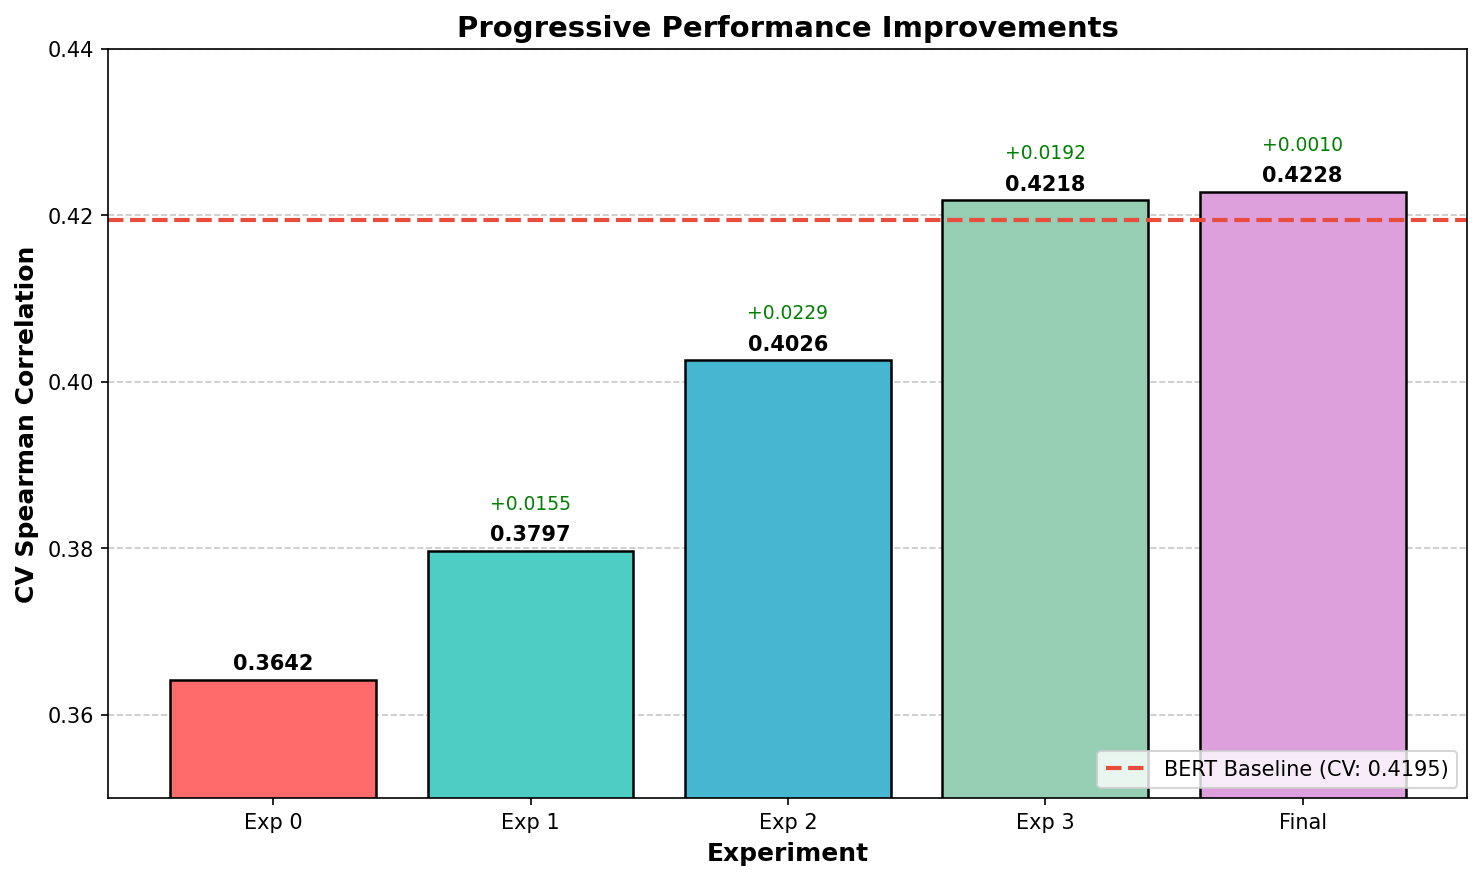
\includegraphics[width=0.9\textwidth]{ablation_chart.png}
    \caption{Progressive CV score improvements across successive experiments. The dashed red line denotes the BERT baseline CV score (0.4195).}
    \label{fig:ablation}
\end{figure}

\paragraph{Analysis of Initial Performance Degradation.}
The substantial performance degradation observed when migrating from BERT to DeBERTa (0.4195 $\rightarrow$ 0.3642) resulted from \textbf{multiple simultaneous changes} during the migration process, encompassing model architecture, tokenization, pooling strategy, and hyperparameter settings. We identify two contributing factors and validate one through controlled experimentation:

\textbf{Potential Factor: Pooling Mismatch.} The baseline explicitly extracts \texttt{[CLS]} and \texttt{[SEP]} token embeddings, thereby encoding the structural boundary between question and answer segments. Our initial DeBERTa configuration employed a different pooling approach, potentially discarding segment-boundary information. \textit{This factor was not validated through controlled ablation in the present study.}

\textbf{Validated Factor: Context Length Sensitivity.} DeBERTa's disentangled attention mechanism relies on relative positional information computed across the full input sequence. Truncating inputs to 512 tokens disrupts the long-range dependencies that DeBERTa was specifically designed to capture. \textbf{This factor is directly validated by Exp~1}: extending the sequence length from 512 to 1024 tokens yielded a +0.0155 improvement in CV score.

These findings underscore that migration to a more expressive architecture necessitates careful adaptation of multiple components. Subsequent experiments systematically addressed each factor, with context length extension and loss function optimization yielding the most substantial validated performance gains.


\section{Discussion}

\subsection{Discrepancy between CV and LB}
As shown in Table \ref{tab:results}, a notable discrepancy emerges: our final single-model CV score (\textbf{0.4228}) exceeds the baseline (0.4195), yet our Private Leaderboard (LB) score (0.4066) falls below the baseline (0.4123).

The competition enforces a strict 2-hour inference limit. The baseline leverages the lightweight \texttt{bert-base-uncased} (110M parameters), enabling \textbf{Snapshot Ensembling} [8]---averaging predictions from over 30 checkpoints within this constraint. Ensembling substantially improves generalization and reduces variance.

In contrast, our DeBERTa-v3-Large (435M parameters) incurs substantially higher computational cost. The 2-hour constraint restricted us to a \textbf{single model}. Although this model demonstrates superior representational quality (as evidenced by higher CV), it lacks the variance-reduction benefits of ensembling.

\subsection{Limitations}
Our approach has the following limitations:
\begin{itemize}
    \item \textbf{Inference Time Constraint:} The 2-hour inference limit precluded checkpoint ensembling, likely contributing to the CV-LB score discrepancy.
    \item \textbf{Limited Baseline Comparison:} Comparison was limited to the 23rd-place solution; evaluation against top-10 solutions would provide broader context.
    \item \textbf{No Post-Processing:} Unlike the baseline, which employs LightGBM stacking [10], we did not apply post-processing.
    \item \textbf{Incomplete Ablation Study:} Due to the rapid iteration inherent in competition settings, controlled single-variable ablations were not conducted for all factors (e.g., pooling strategy in isolation). Consequently, the reported performance improvements reflect cumulative rather than isolated changes.
\end{itemize}

\begin{figure}[h]
    \centering
    
\includegraphics[width=0.8\textwidth]{lb_screenshot.png}
    \caption{Kaggle Private Leaderboard showing our final submission ranking.}
    \label{fig:lb_score}
\end{figure}


\section{Conclusion}

This work demonstrates that adopting a modern backbone (DeBERTa-v3-Large) and aligning training objectives with the ranking nature of the evaluation metric are critical for improving performance on the Google QUEST Q\&A Labeling challenge. Our principal findings are as follows:

\begin{enumerate}
    \item \textbf{Metric-aligned optimization is essential:} Replacing BCE with Ranking + Soft Spearman loss substantially improves Spearman correlation.
    \item \textbf{Context length is critical:} Extending maximum sequence length from 512 to 1024 tokens prevents information loss in longer Q\&A pairs.
    \item \textbf{Architecture migration requires systematic adaptation:} Simply substituting a more expressive backbone is insufficient; context length and training objectives must be co-optimized for the target task.
\end{enumerate}

While our single-model CV (0.4228) surpasses the baseline (0.4195), the Private LB score (0.4066) is lower than the baseline (0.4123) due to inference time constraints. Future work may explore model distillation or quantization to enable efficient checkpoint ensembling within the 2-hour limit.


\begin{ack}
This work was completed as the \textbf{final term project} for the Natural Language Processing course under the \textbf{Artificial Intelligence for Natural Language Technology Program} offered by the \textbf{Taiwan Artificial Intelligence College Alliance (TAICA)}. The course was hosted by National Tsing Hua University (NTHU) and instructed by \textbf{Prof. Hung-Yu Kao}. We thank the instructor and teaching assistants for their guidance and feedback.

Experiments were conducted on a workstation with two NVIDIA RTX PRO 6000 Blackwell GPUs (96 GB VRAM each). We also acknowledge the use of Kaggle Notebooks for inference submissions.
\end{ack}

\section*{References}
% References follow the acknowledgments.
% You can use BibTeX or manual references.

{\small

[1] He, P., Gao, J., \& Chen, W. (2023). DeBERTaV3: Improving DeBERTa using ELECTRA-Style Pre-Training with Gradient-Disentangled Embedding Sharing. In {\it International Conference on Learning Representations}. \url{https://openreview.net/forum?id=sE7-XhLxHA}

[2] Devlin, J., Chang, M.-W., Lee, K., \& Toutanova, K. (2019). BERT: Pre-training of Deep Bidirectional Transformers for Language Understanding. In {\it Proceedings of NAACL-HLT}, pp.\ 4171--4186. \url{https://aclanthology.org/N19-1423}

[3] Liu, Y., Ott, M., Goyal, N., Du, J., Joshi, M., Chen, D., Levy, O., Lewis, M., Zettlemoyer, L., \& Stoyanov, V. (2019). RoBERTa: A Robustly Optimized BERT Pretraining Approach. {\it arXiv preprint arXiv:1907.11692}.

[4] Blondel, M., Teboul, O., Berthet, Q., \& Djolonga, J. (2020). Fast Differentiable Sorting and Ranking. In {\it Proceedings of ICML}, pp.\ 950--960. \url{https://arxiv.org/abs/2002.08871}

[5] Loshchilov, I., \& Hutter, F. (2019). Decoupled Weight Decay Regularization. In {\it International Conference on Learning Representations}. \url{https://openreview.net/forum?id=Bkg6RiCqY7}

[6] Sun, C., Qiu, X., Xu, Y., \& Huang, X. (2019). How to Fine-Tune BERT for Text Classification? In {\it Chinese Computational Linguistics}, pp.\ 194--206. Springer.

[7] Peters, M., Neumann, M., Iyyer, M., Gardner, M., Clark, C., Lee, K., \& Zettlemoyer, L. (2018). Deep Contextualized Word Representations. In {\it Proceedings of NAACL-HLT}, pp.\ 2227--2237. \url{https://aclanthology.org/N18-1202}

[8] Huang, G., Li, Y., Pleiss, G., Liu, Z., Hopcroft, J. E., \& Weinberger, K. Q. (2017). Snapshot Ensembles: Train 1, Get M for Free. In {\it International Conference on Learning Representations}. \url{https://openreview.net/forum?id=BJYwwY9ll}

[9] Inoue, H. (2019). Multi-Sample Dropout for Accelerated Training and Better Generalization. {\it arXiv preprint arXiv:1905.09788}.

[10] Ke, G., Meng, Q., Finley, T., Wang, T., Chen, W., Ma, W., Ye, Q., \& Liu, T.-Y. (2017). LightGBM: A Highly Efficient Gradient Boosting Decision Tree. In {\it Advances in Neural Information Processing Systems}, vol.\ 30, pp.\ 3146--3154.

[11] Google. (2020). Google QUEST Q\&A Labeling. {\it Kaggle Competition}. \url{https://www.kaggle.com/competitions/google-quest-challenge}
}

%%%%%%%%%%%%%%%%%%%%%%%%%%%%%%%%%%%%%%%%%%%%%%%%%%%%%%%%%%%%

\end{document}